\chapter{Einleitung}
\label{Einleitung}
Im Rahmen der Vorlesung \textit{Webprogrammierung} galt es als Projekt, eine Website zu erstellen, welche ein Schulsportfest in freier Art und Weise unterstützt. Dabei mussten verschiedene Technologien aus dem Bereich der Webprogrammierung eingesetzt werden, um für diese eine Grundverständnis zu entwickeln.
\par
Die in dieser Ausarbeitung behandelte Internetseite unterstützt Teilnehmer und Teilhaber vor, während und nach dem Fest: So kann sich z.B. ein Auswärtiger vor oder am Tage des Sportfestes eine Anfahrtsbeschreibung anschauen, Wettkämpfer können danach eigene Bestwerte betrachten. Und entstandene Fotos sind in einer Galerie für jedermann zugänglich.
\par
Diese Arbeit beschreibt die benutzten und geforderten Technologien, indem zuerst jene der Benutzeroberfläche erläutert werden. Danach werden die Technologien für die Client-Server-Architektur durchleuchtet.

\chapter{Benutzeroberfläche}
\label{Benutzeroberfläche}

\section{HTML zur Erstellung der Website}
\label{HTML zur Erstellung der Website}
Das Grundgerüst der kompletten Benutzeroberfläche bildet eine \textit{"'index.html"'}-Datei. Als One-Pager ist sie die einzige HTML-Datei und beinhaltet somit sämtliche Anzeige- und Steuerelemente des Projektes.
\par
Dazu zählen:
\begin{itemize}
	\item eine Navigationsbar
	\item ein Banner
	\item eine Übersicht der Wettkämpfe und Dialoge zur Anzeige der Wettkampfergebnisse
	\item eine filterbare Galerie
	\item eine Anfahrtsbeschreibung mit Google Maps
	\item Kontaktinformationen
	\item ein Bereich für den Log In und die Registrierung \item ein kleines Spiel zum Zeitvertreib
	\item das Heise Plug-In für Social Buttons
	\item ein Footer mit der Serverzeit	
\end{itemize}
Auf viele dieser Punkte wird im weiteren Verlauf der Arbeit eingegangen. Zudem befinden sich im Anhang Bilder von den Bereichen der Seite, welche nicht genauer behandelt werden.

\section{CSS}
\label{CSS}
\subsection{Bootstrap}
\label{Bootstrap}
Zur optischen Verschönerung der Seite wurde das CSS-Framework Bootstrap von Twitter eingebunden, was durch ein \textit{<script>}-Tag im \textit{<head>} importiert wurde. Angewendet wird das Framework dann durch Benutzen seiner CSS-Klassen auf das gewünschte HTML-Element. Bspw. lassen sich durch die Klasse \textit{"'btn-lg"'} visuell ansprechende, große, farbige Buttons mit sattem Text und abgerundeten Ecken erzeugen (auch zu sehen in Abbildung \vref{fig:responsive}).
\par
Darüber hinaus wurden für dieses Projekt auch eigene CSS-Klassen geschrieben, auf welche an dieser Stelle aber nicht genau eingegangen werden.

\subsection{Kompatibilität mit mobilen Endgeräten}
\label{Kompatibilität mit mobilen Endgeräten}
Ein weiterer Vorteil des Twitter Bootstrap Frameworks ist, dass die Website \textit{"'responsive"'} ist, was bedeutet, dass sich die Seite der Fenstergröße anpasst. Dadurch ist sie auch für mobile Endgeräte kompatibel: Bei Verkleinerung des Fensters ordnen sich die Seitenelemente automatisch neu an und die Navigationsbar oben wird durch einen Menü-Button komprimiert (siehe Abbildung \vref{fig:responsive}).

\begin{figure}[!h]
	\makebox[\textwidth]{ 
		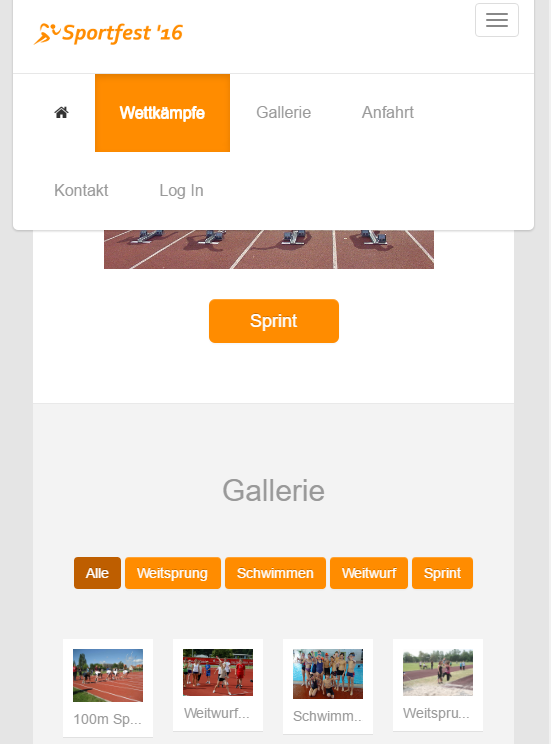
\includegraphics[scale=0.5]{img/responsive.png}}
	\caption{Responsive Design der Seite}
	\label{fig:responsive}
\end{figure}

\section{Clientseitiges JavaScript für benutzerspezifische Seiteninhalte}
\label{Clientseitiges JavaScript}
Um Frontend-seitige Anpassungen der Website vorzunehmen, ohne die komplette Seite neu laden zu müssen, wird JavaScript verwendet. In diesem Projekt wird es unter anderem angewandt, um zu überprüfen, ob ein Nutzer angemeldet ist, und um daraus resultierend Wettkampfergebnisse des angemeldeten Benutzers anzuzeigen.
\par
Durch Klicken auf den Knopf für die Ergebnisse wird dabei nicht nur ein Dialog geöffnet, sondern auch eine Funktion aufgerufen (siehe Abbildung \vref{fig:javaScript}). Die globalen Variablen, welche in dieser Funktion benutzt werden, sind beim Aufruf der Seite \textit{null}, und werden erst nach erfolgreicher Anmeldung des Nutzers mit einem Wert belegt (siehe auch Kapitel \vref{Konsumieren der Daten im Frontend per AJAX-Call}).

\begin{figure}[!h]
	\makebox[\textwidth]{ 
		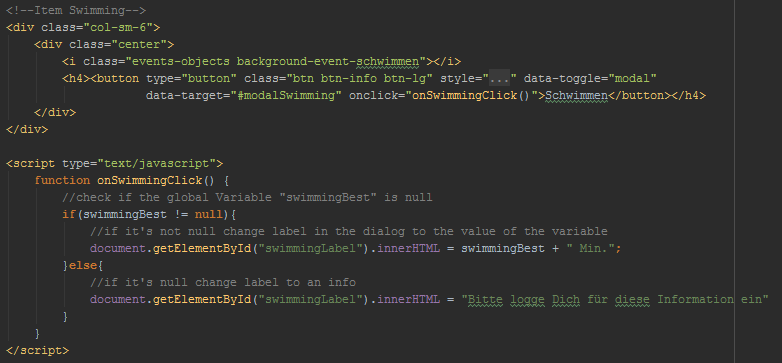
\includegraphics[scale=0.8]{img/javaScript.png}}
	\caption{Skript zur Darstellung der Wettkampfergebnisse}
	\label{fig:javaScript}
\end{figure}

\section{Anfahrtsbeschreibung per Google Maps}
\label{Anfahrtsbeschreibung per Google Maps}
Für den Fall, dass der Nutzer der Website von außerhalb des Ortes der Schule kommt, wurde eine Anfahrtsbeschreibung mittels der Google Maps API eingebunden (siehe Abbildung \vref{fig:googleMaps}).

\begin{figure}[!hp]
	\makebox[\textwidth]{ 
		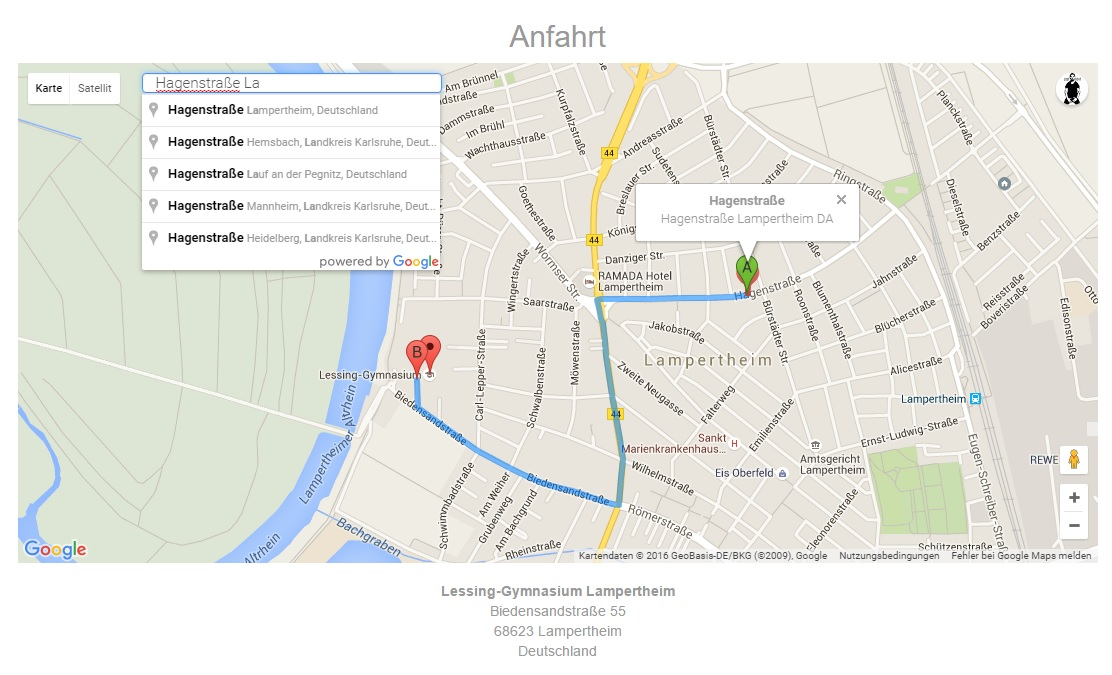
\includegraphics[scale=0.5]{img/googleMaps.jpg}}
	\caption{Anfahrtsbeschreibung mit Google Maps}
	\label{fig:googleMaps}
\end{figure}

Auf dem Bild ist nicht nur der Standort der Schule vermerkt, sondern darüber hinaus kann der User über ein Eingabefeld links oben seine Abfahrtsadresse eingeben, sodass die optimale Route auf der Karte angezeigt wird. Des Weiteren wurde mit Hilfe der Autocomplete-Funktion der Google Maps API eine automatische Vervollständigung der Adresse bei Eingabe in das Adressfeld implementiert, wie auf dem Screenshot zu sehen ist.
\par
Verwirklicht wurde die Einbindung, indem zuerst die Google Maps API und die Google Maps API für die Google Places per \textit{<script>}-Tag in den \textit{<head>} der Website importiert wurde (siehe Abbildung \vref{fig:googleMapsAPI}).

\begin{figure}[!hp]
	\makebox[\textwidth]{ 
		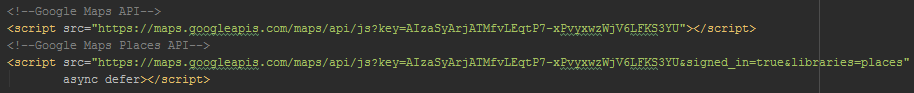
\includegraphics[scale=0.8]{img/googleMapsAPI.png}}
	\caption{API Einbindung von Google Maps}
	\label{fig:googleMapsAPI}
\end{figure}

Danach wird über eine JavaScript-Funktion, ebenfalls im \textit{<head>}-Bereich die Map erstellt (siehe Abbildung \vref{fig:googleMapsInit}).

\begin{figure}[!h]
	\makebox[\textwidth]{ 
		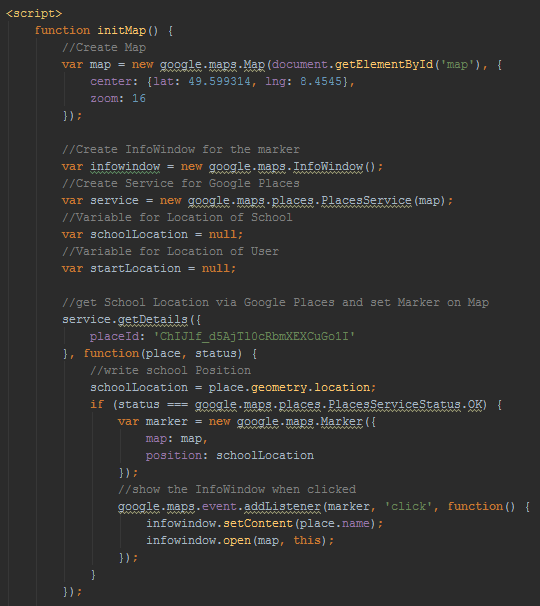
\includegraphics[scale=1]{img/googleMapsInit.png}}
	\caption{\textit{initMap}-Funktion zur Erstellung der Karte}
	\label{fig:googleMapsInit}
\end{figure}

Im zweiten Teil derselben Funktion wird die Autocomplete-Funktion für das Input-Feld implementiert und der Marker für die eingegebene Adresse auf der Karte gesetzt (siehe Abbildung \vref{fig:googleMapsInit2}).

\begin{figure}[!h]
	\makebox[\textwidth]{ 
		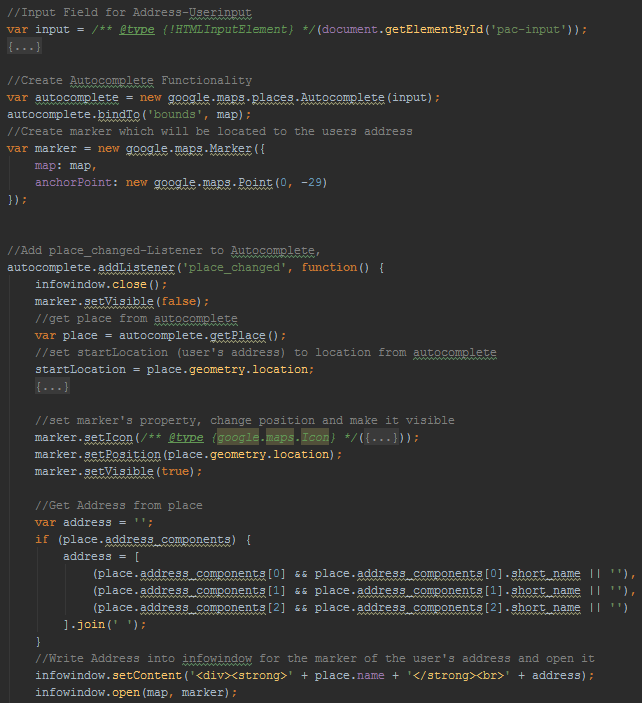
\includegraphics[scale=1]{img/googleMapsInit2.png}}
	\caption{Autocomplete-Funktion und Adressmarker}
	\label{fig:googleMapsInit2}
\end{figure}

Die Route zwischen der Abfahrtsadresse und der Schule wird im letzten Teil der Funktion erstellt und angezeigt. Vor Schließen des \textit{<script>}-Tags wird noch ein Event-Listener hinzugefügt, welcher auf das Aufrufen der Seite wartet und bei diesem dann die Karte zeichnet, indem die Funktion \textit{initMap} ausgeführt wird (siehe Abbildung \vref{fig:googleMapsInit3}).

\begin{figure}[!h]
	\makebox[\textwidth]{ 
		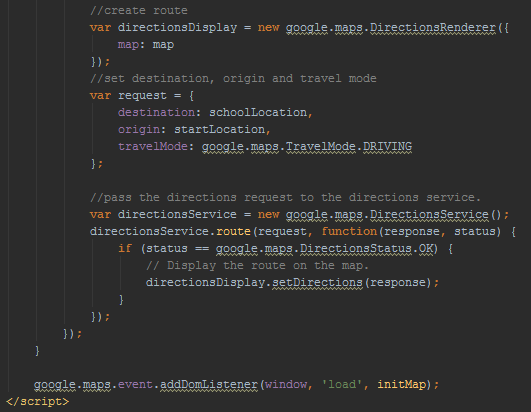
\includegraphics[scale=1]{img/googleMapsInit3.png}}
	\caption{Routenerstellung}
	\label{fig:googleMapsInit3}
\end{figure}

Um nun die Karte auch tatsächlich in der Website anzeigen zu können, wurde zu guter Letzt noch ein \textit{div}-Container mit der Id \textit{"'map"'} an der gewünschten Stelle erstellt (siehe Abbildung \vref{fig:googleMapsDiv}). Dieses \textit{div} wird dann durch die Funktion \textit{initMap} gefüllt. Dafür wird bei Deklaration der Karte über einen Id-Selektor das entsprechende \textit{div} ausgewählt, in welchem die Google Map erscheinen soll (siehe ganz oben in Abbildung \vref{fig:googleMapsInit}).

\begin{figure}[!h]
	\makebox[\textwidth]{ 
		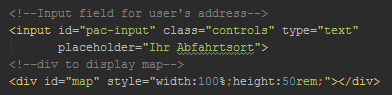
\includegraphics[scale=1]{img/googleMapsDiv.png}}
	\caption{Container für die Karte}
	\label{fig:googleMapsDiv}
\end{figure}

\section{Canvas-Minispiel}
Mittels Canvas wurde ein kleines Spiel f\"ur den Zeitvertreib implementiert. Dabei wurden zuerst ein Canvas-Element und grundlegende Funktionen definiert um z.B. den Inhalt des Canvas-Elements zu löschen, diese Funktion wird mittels \textit{setInterval} immer wieder aufgerufen, damit das Canvas neu gezeichnet werden kann.     
\newline
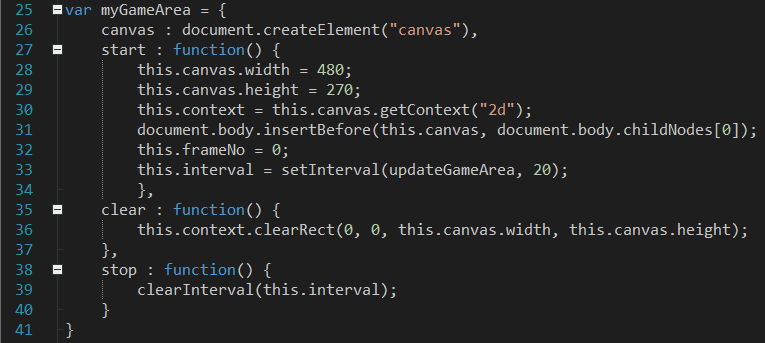
\includegraphics[width=1\textwidth]{img/vincent/abb04.png}
\newline
Durch die \textit{Component}-Funktion werden die Objekte, wie z.B. der Hintergrund und der Taucher erzeugt, dabei werden Bilddateien geladen, wie in folgender Abbildung zu erkennen ist: 
\newline
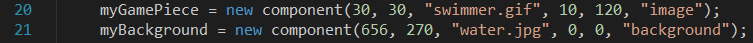
\includegraphics[width=1\textwidth]{img/vincent/abb05.png}
\newline
Die \textit{Component}-Funktion erh\"alt als Parameter die Koordinatenposition des \"ubergebenen Elements. Wenn es sich um ein Bild handelt, wird mittels \textit{new Image()} dieses zum Zeichnen auf dem Canvas erstellt. In der \textit{Update}-Funktion wird das Bild letztendlich gezeichnet. Da diese Funktion mehrmals die Sekunde aufgerufen wird, entsteht die Illusion einer Bewegung des Tauchers und des Hintergrundes. Dabei wird mittels der \textit{newPos}-Funktion daf\"ur Sorge getragen, dass sich die logische Position des Bildes ver\"andert, die Variable \textit{speedY} und \textit{speedX} geben die Geschwindigkeit an, mit der die Position ver\"andert wird. 
\newline
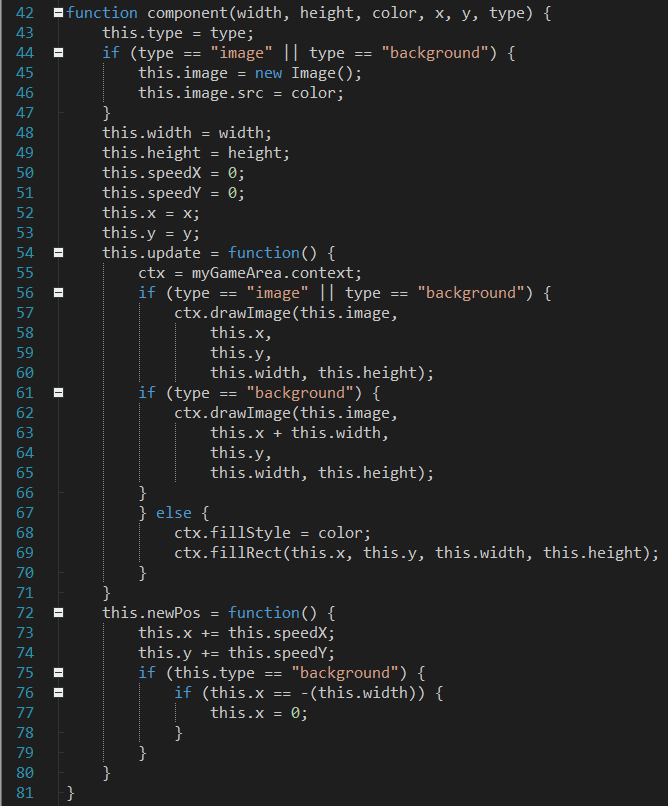
\includegraphics[width=1\textwidth]{img/vincent/abb06.png}
\newline
Den Motor des Programms bildet die \textit{updateGameArea}-Funktion. Sie wird per \textit{setInterval} alle 20 Millisekunden aufgerufen und aktualisiert die Position des Hintergrunds und die des Tauchers, außerdem sorgt sie daf\"ur, dass die \textit{Update}-Funktionen ausgef\"uhrt werden:
\newline
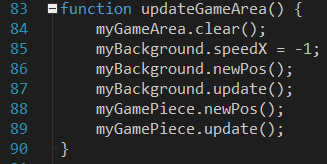
\includegraphics[width=0.6\textwidth]{img/vincent/abb07.png}
\newline
Der User kann die Bewegung des Tauchers per Button steuern, dabei wird die Geschwindigkeit des Tauchers, je nachdem, welcher Button gedr\"uckt wurde, entsprechend ver\"andert:
\newline
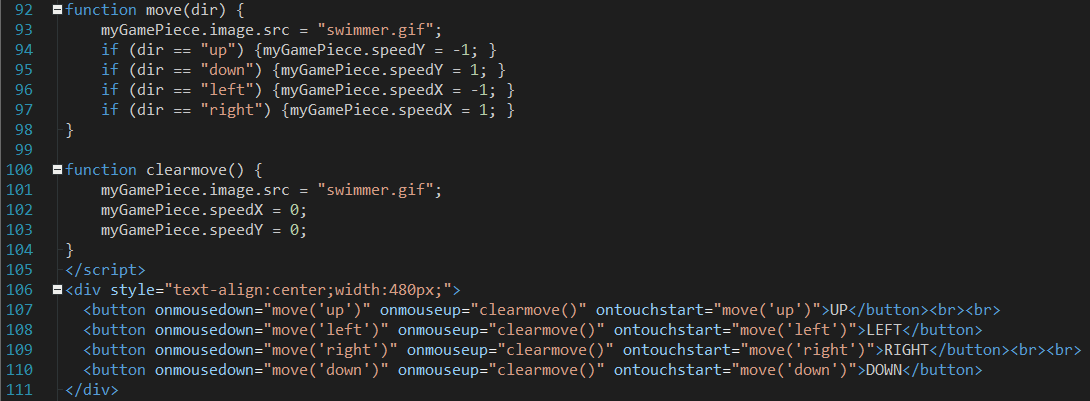
\includegraphics[width=1\textwidth]{img/vincent/abb08.png}
\newline
Das Endergebnis ist in nachfolgender Abbildung visualisiert:
\newline
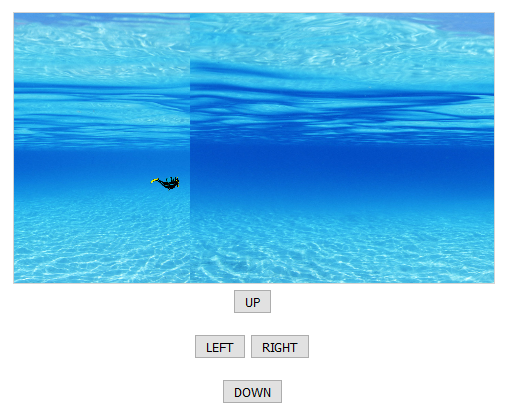
\includegraphics[width=0.7\textwidth]{img/vincent/abb09.png}
\newline

\section{Einbindung von Social Buttons mittels des Heise Plug-Ins}
\label{Einbindung von Social Buttons mittels des Heise Plug-Ins}
Um soziale Netzwerke der Schule oder des Sportfestes auf der Seite verlinken zu können, wurden mittels des Heise Plug-Ins Social Buttons eingebunden (Facebook, Twitter und Google+). Der Vorteil bei diesem Plug-In liegt darin, dass der Nutzer selbst bestimmen kann, ob er diese Buttons benutzen möchte oder komplett für die Seite deaktivieren will. Der tiefere Sinn liegt in der Datenschutzproblematik bei der Einbindung der "`Like"'-Buttons von Facebook und Co.: Das Einbinden dieser Buttons erfolgt über einen iFrame, welcher von Facebook und Co. selbst zur Verfügung gestellt wird. Der iFrame enthält Code, der veranlasst, dass die URL oder auch Cookies der aufgerufenen Seite an Facebook geschickt werden. Ist der Anwender zudem gleichzeitig in einem anderen Fenster bei Facebook angemeldet, so übermittelt das iFrame zusätzlich Sitzungs-Id, wodurch Facebook einen Webseitenaufruf einer konkreten Person zuordnen kann.
\par
Damit das also nicht passiert, dürfte die Seite entweder keinerlei Elemente von Facebook, Twitter und Google+ beinhalten oder das Heise Plug-In verhindert eben genau dies, indem all diese Elemente zunächst bei Aufruf der Seite deaktiviert sind. Möchte der Nutzer nun eine der Funktionen der sozialen Netzwerke nutzen, so muss er sie zuvor über das Plug-In aktivieren.
\par
In die Website integriert wurde das Plug-In, indem zuerst das von Heise zur Verfügung gestellte Skript des Plug-Ins im \textit{<head>} geladen wird und ein HTML-Element durch ein weiteres Skript gefüllt wird (siehe Abbildung \vref{fig:heisePlugin1}).

\begin{figure}[!h]
	\makebox[\textwidth]{ 
		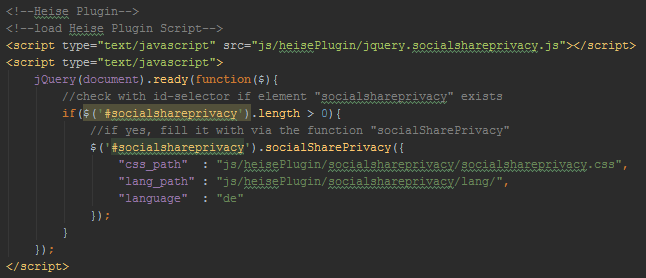
\includegraphics[scale=1]{img/heisePlugin1.png}}
	\caption{Integrieren des Heise Plug-Ins}
	\label{fig:heisePlugin1}
\end{figure}

Durch ein \textit{div}-Element mit Id \textit{"'socialshareprivacy"'} vor dem Footer der Seite (wie es in Abbildung \vref{fig:heisePlugin1} selektiert wird) wird das Plug-In dann am Ende der Seite angezeigt (siehe Abbildung \vref{fig:heisePlugin2}).

\begin{figure}[!h]
	\makebox[\textwidth]{ 
		
\includegraphics[scale=1]{img/heisePlugin2.png}}
	\caption{Heise Plug-In in der Website}
	\label{fig:heisePlugin2}
\end{figure}

\chapter{Client-Server-Architektur}
\label{Client-Server-Architektur}

\section{Registrierung mit PHP}
Die Registrierung eines Users wurde mit PHP umgesetzt, dabei wurde zuerst ein einfaches HTML-Formular erstellt, um die vom User eingegebenen Registrierungsdaten an den Server zu \"ubertragen, wobei es ebenfalls zur Auswertung des HTML-Formulars durch den Server kommt. 
Das nachfolgende Listing zeigt das HTML-Formular:
\newline
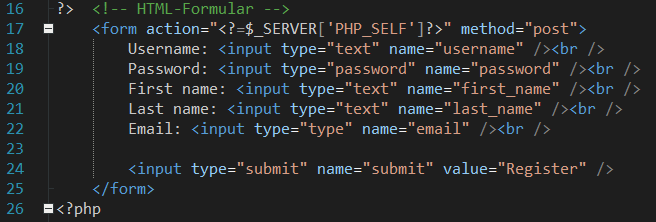
\includegraphics[width=1\textwidth]{img/vincent/abb11.png}
\newline
Wie aus dem Code zu entnehmen ist, werden f\"ur die Registrierung Username, Passwort, Vor- und Zuname und die Email-Adresse des Users \"ubertragen. Durch die Definition des Passworts Eingabefeld mit \textit{type="password"} wird ein Maskieren der eingegebenen Zeichen mit Punkten erreicht, wie folgende Abbildung zeigt:
\newline
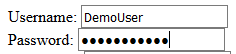
\includegraphics[width=0.5\textwidth]{img/vincent/abb01.png}
\newline
Nachdem der User seine Daten zur Registrierung eingegeben hat, werden diese an den Server gesendet. Der Server baut eine Verbindung zur \textit{MySQL}-Datenbank auf, dabei greift er auf eine zuvor erstellte Konfigurationsdatei zurück und liest die ben\"otigten Informationen, wie z.B. den Datenbankuser und dessen Passwort. Anschlie{\ss}end wird die Verbindung zur Datenbank \"uberpr\"uft. Das nachfolgende Listing zeigt die beschriebene Funktion:
\newline
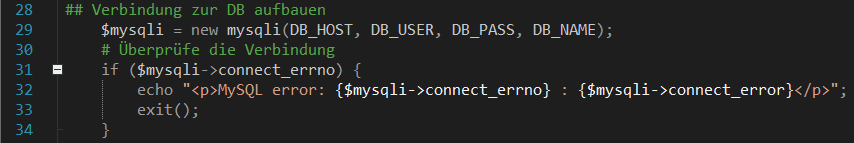
\includegraphics[width=1\textwidth]{img/vincent/abb12.png}
\newline

Nachdem die Verbindung zur Datenbank \"uberpr\"uft wurde, wird eine Datenbankabfrage vorbereitet, dabei werden die Daten des HTML-Formulars in Variablen gespeichert. Nun wird mittels einer Else-If-Verzweigung \"uberpr\"uft, ob ein User mit demselben Usernamen oder derselben Email-Adresse bereits existiert, damit sich kein User mit demselben Informationen ein weiteres Mal registrieren kann und die Datenkonsistenz gew\"ahrleistet ist. Durch das \textit{echo}-Kommando wird eine entsprechende Information ausgegeben, sollte es bereits existente Eintr\"age geben. Folgendes Listing zeigt den beschriebenen Code:
\newline	
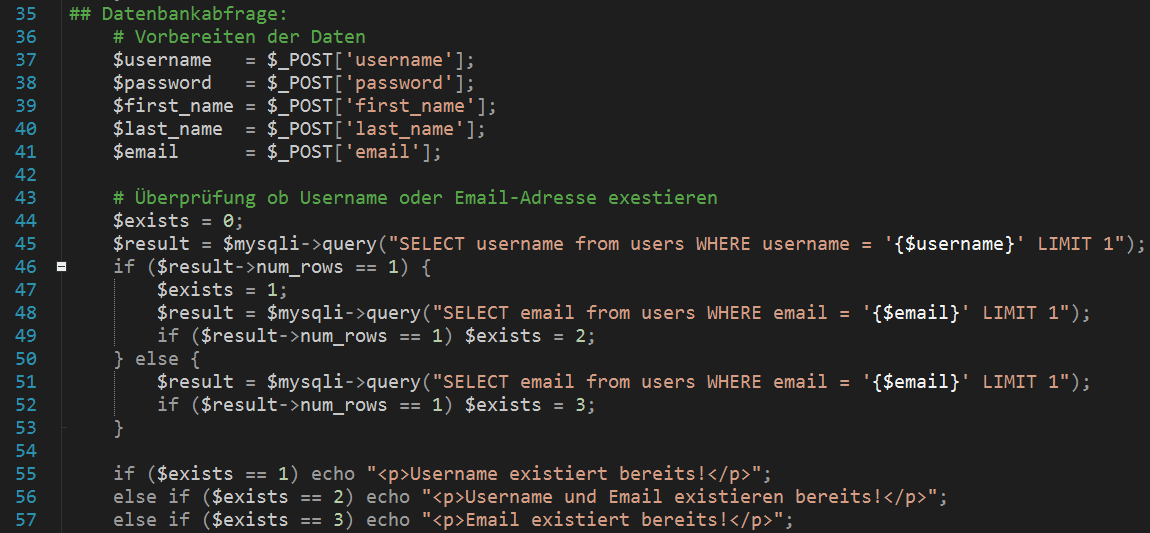
\includegraphics[width=1\textwidth]{img/vincent/abb13.png}
\newline

Nachdem sichergestellt wurde, dass die Daten f\"ur die Erstellung eines neuen Users geeignet sind, wird ein neuer Datenbankeintrag mit den Daten aus dem HTML-Formular erstellt. Anschlie{\ss}end wird eine Meldung ausgegeben, welche dem User mitteilt, das die Registrierung erfolgreich war:
\newline	
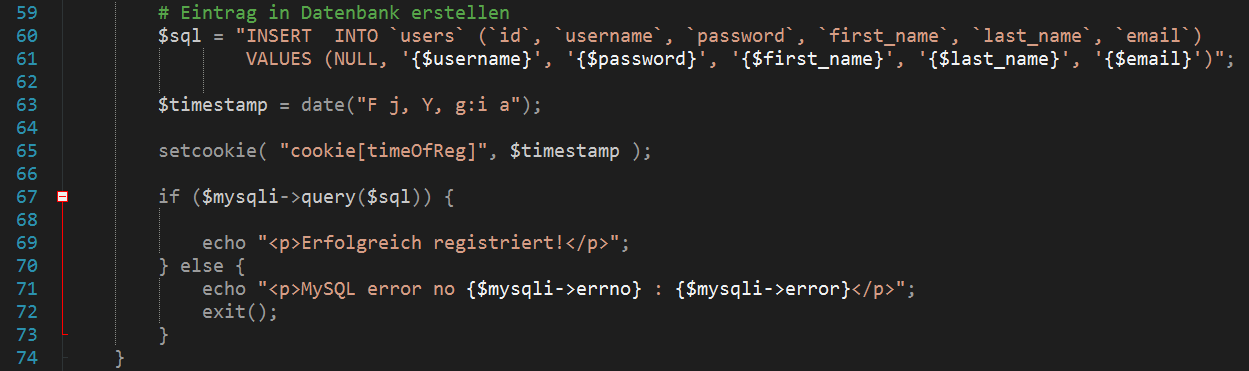
\includegraphics[width=1\textwidth]{img/vincent/abb14.png}
\newline
Im Coding wird auch ein Cookie gesetzt, dazu mehr im Abschnitt, welcher sich mit dem Setzen und der Auswertung eines Cookies besch\"aftigt.	

\section{Anmeldefunktion mit node.js und AJAX-Call}
\label{Anmeldefunktion mit node.js und AJAX-Call}
Ist ein Nutzer der Website gleichzeitig auch Teilnehmer des Sportfestes, was zugleich bedeutet, dass für ihn Ergebnisse für Weitsprung, Sprint etc. in der Datenbank hinterlegt sind, kann er sich jene Ergebnisse anzeigen lassen, indem er sich anmeldet. Um diese Information von der Datenbank an das Frontend kommunizieren zu können, bedarf es eines Servers, der sich mit der Datenbank verbindet, und einer Technologie, welche sich die benötigten Informationen von dem Server holt und an das Frontend bringt. 
\par
Für diese Website wurde Ersteres mit einem REST-Service durch node.js und das Zweite mit einem jQuery AJAX-Call realisiert, der den REST-Service konsumiert.

\subsection{Bereitstellung eines REST-Service durch node.js}
\label{Bereitstellung eines REST-Service durch node.js}
Die Anbindung der MySQL-Datenbank wurde in node.js mit Hilfe des Plug-Ins \textit{express} und \textit{mysql} verwirklicht. Nach deren Einbindung wird eine Datenbankverbindung aufgebaut und ein REST-Service erstellt, welcher sich über die URL \textit{"'localhost:3000/getUser/[username]/[password]"'} als GET-Request aufrufen lässt. Der Aufruf gibt dann die kompletten Userinfos als JSON-Objekt zurück (siehe Abbildung \vref{fig:nodeServer1}).

\begin{figure}[!h]
	\makebox[\textwidth]{ 
		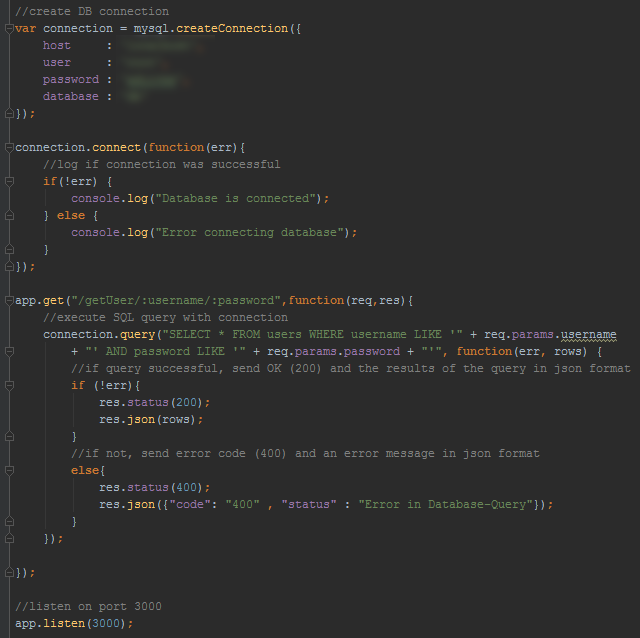
\includegraphics[scale=1]{img/nodeServer1.png}}
	\caption{Datenbankverbindung und REST-Service im node.js-Server}
	\label{fig:nodeServer1}
\end{figure}

Zusätzlich wurde noch vor der Erstellung der Datenbankanbindung ein besonderer HTTP-Header erstellt, um das Cross-Origin-Problem zu beheben, durch welches manche Browser AJAX-Calls unterbinden, welche auf externe APIs/ Server zugreifen (siehe Abbildung \vref{fig:nodeServer2}).

\begin{figure}[!h]
	\makebox[\textwidth]{ 
		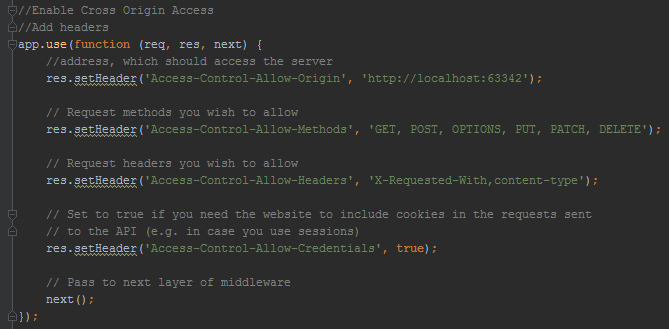
\includegraphics[scale=1]{img/nodeServer2.png}}
	\caption{Erstellen des Headers für Cross-Origin-Aufrufe}
	\label{fig:nodeServer2}
\end{figure}

\subsection{Konsumieren der Daten im Frontend per AJAX-Call}
\label{Konsumieren der Daten im Frontend per AJAX-Call}

Meldet der Nutzer sich nun über folgendes Log-In-Fenster im unteren Teil der Website an...

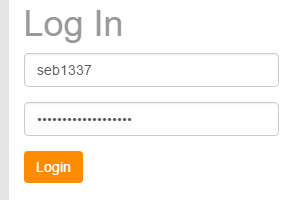
\includegraphics[scale=0.5]{img/logIn.png}

...so kann er sich seine Wettkampfergebnisse anzeigen lassen (siehe Abbildung \vref{fig:wettkampfErgebnisse}).
\begin{figure}[!h]
	\makebox[\textwidth]{ 
		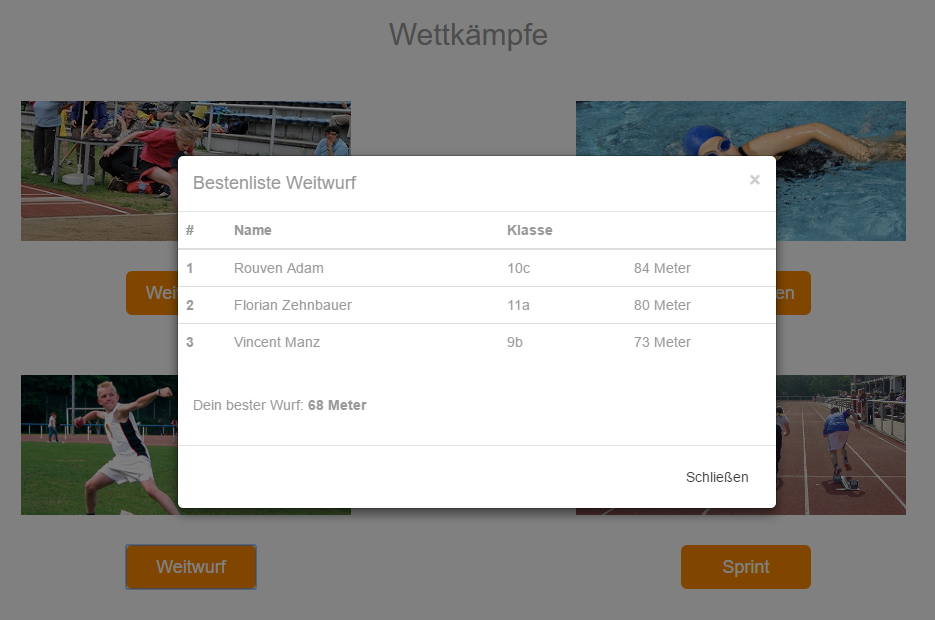
\includegraphics[scale=0.55]{img/wettkampfErgebnisse.png}}
	\caption{Wettkampfergebnisse-Dialog}
	\label{fig:wettkampfErgebnisse}
\end{figure}

Dies geschieht durch einen AJAX-Call, welcher bei der Anmeldung ausgeführt wird (siehe Abbildung \vref{fig:ajaxCall}).

\begin{figure}[!h]
	\makebox[\textwidth]{ 
		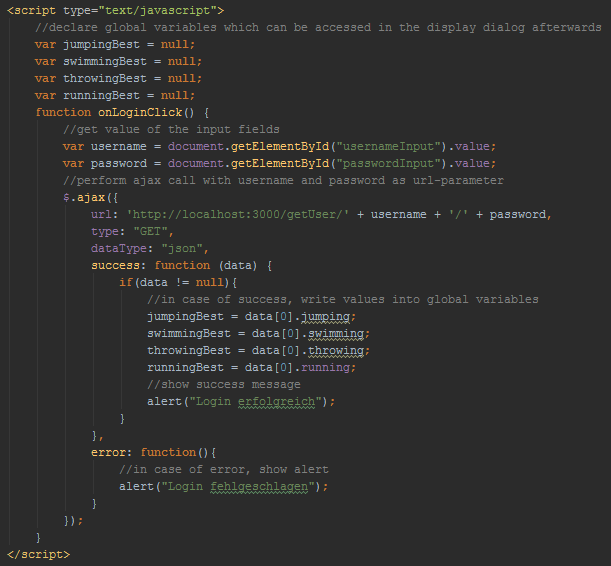
\includegraphics[scale=1]{img/ajaxCall.png}}
	\caption{AJAX-Call}
	\label{fig:ajaxCall}
\end{figure}

Durch den AJAX-Call werden globale JavaScript Variablen gesetzt, welche dann bei Aufruf des Dialogs abgefragt werden. Sind die Variablen bei Dialogaufruf leer bzw. ist der Nutzer nicht eingeloggt, so steht anstelle seines Wettkampfergebnisses ein Hinweis, dass der User sich für diese Information anmelden muss (siehe auch Kapitel \vref{Clientseitiges JavaScript}).

\pagebreak
\section{Websockets zur Systemzeitabfrage}
Eines der Ziele des Projekts war die Implementierung von Websockets, diese wurde mittels \textit{node.js} und der Bibliothek \textit{node.js-websocket}
auf der Serverseite und mittels JavaScript auf der Clientseite umgesetzt. Der Server horcht auf eingehende Verbindungen auf dem Port 8001. Sobald sich ein Client verbunden hat, wird ein Event gefeuert und der Server sendet seine Systemzeit \"uber die Websocket-Verbindung an den Client, wie aus folgendem Coding zu entnehmen ist:  
\newline
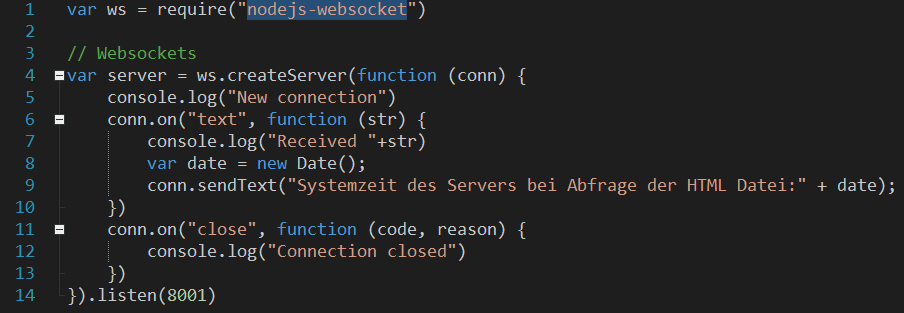
\includegraphics[width=1\textwidth]{img/vincent/abb02.png}
\newline
Auf der Clientseite wird mittels JavaScript ein Websocket erstellt, welcher ebenfalls Events feuert. Sobald die Verbindung aufgebaut ist, wird eine Probenachricht an den Server gesendet. Der Server wiederum sendet seine Systemzeit, diese wird dann mittels \textit{document.getElementById} f\"ur den User im Frontend dargestellt: 
\newline
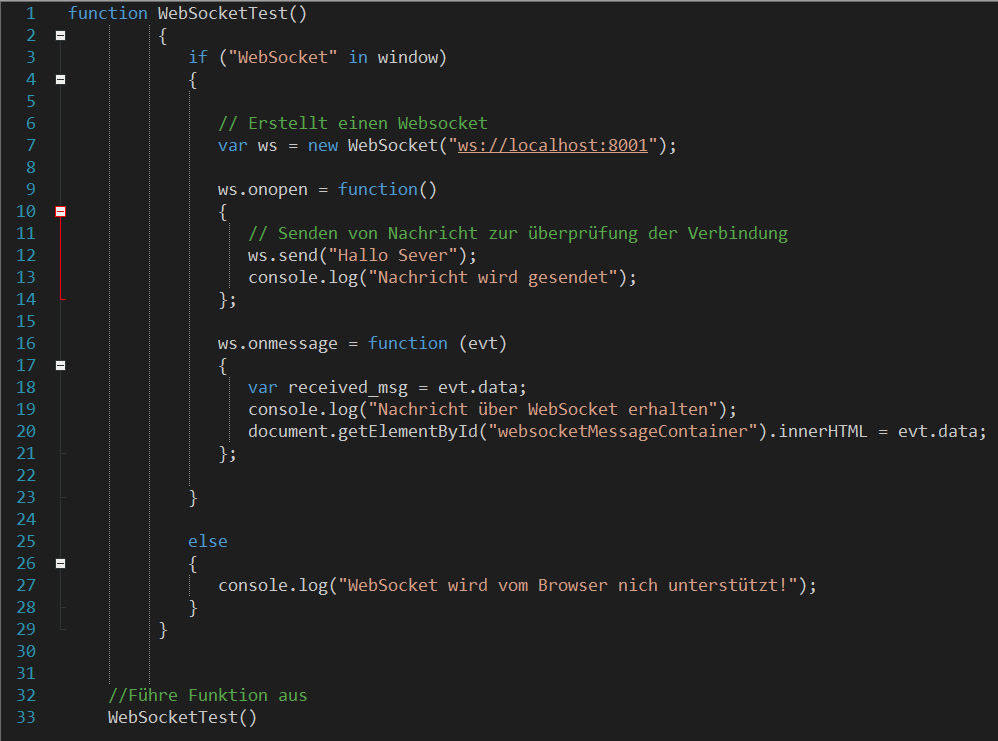
\includegraphics[width=1\textwidth]{img/vincent/abb03.png}
\newline
Das Ergebnis sieht wie folgt aus:
\newline

\includegraphics[width=1\textwidth]{img/vincent/abb17.png}
\newline

\section{Serverseitige Bildgenerierung}
Um die serverseitige Bildgenerierung mittels php durchzuf\"uhren, wurde eine neue php-Datei erstellt. Diese soll bei Aufruf ein Banner erzeugen, welches dann in die Hauptseite eingebunden wird. Dabei wird der Text 'Viel Erfolg bei den Wettk\"ampfen!' verwendet, welcher in zuf\"alliger Farbe angezeigt wird, es wird außerdem ein eigener Font genutzt. Durch die rand Funktion wird ein zuf\"alliger Farbwert generiert und anschließend verwendet, um die Textfarbe festzulegen. Am Anfang wird noch \"uberpr\"uft, ob bereits ein entsprechendes Bild generiert wurde. Wenn dass der Fall ist, wird dieses \"uberschrieben. Dadurch wird dem User bei jedem Aufruf der Seite ein Banner in anderer Farbe angezeigt. Folgendes wurde programmiert:
\newline
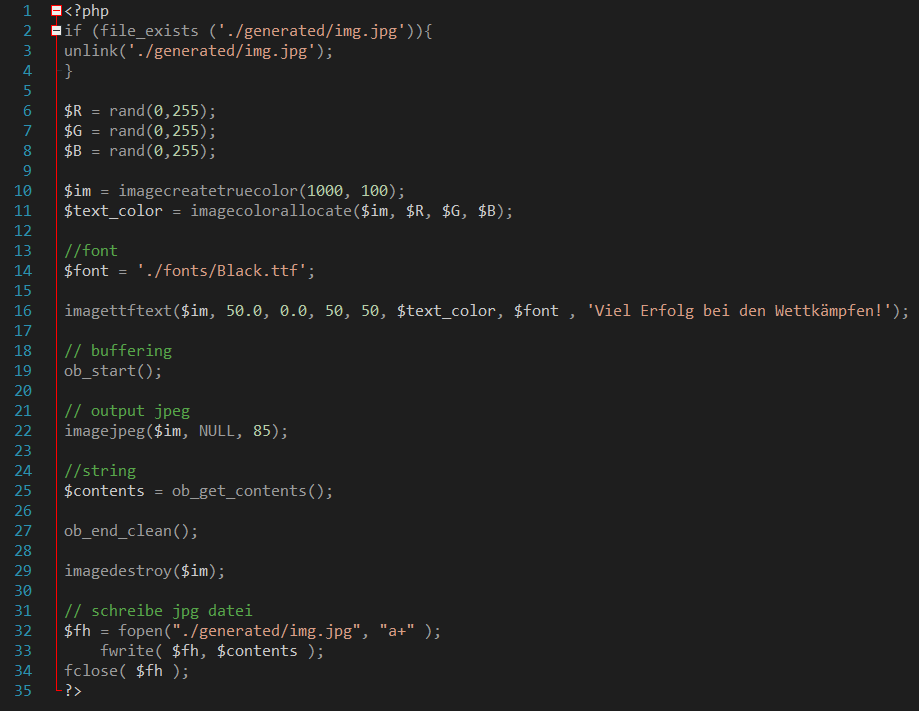
\includegraphics[width=1\textwidth]{img/vincent/abb10.png}
\newline
Hier zwei Beispiele f\"ur das Ergebnis der Generierung:
\newline

\includegraphics[width=1\textwidth]{img/vincent/img.jpg}

\includegraphics[width=1\textwidth]{img/vincent/img2.jpg}
\newline

\section{Cookie für den Registrierungszeitpunkt}
Ein weiteres Ziel des Projektes war die sinnvolle Verwendung eines Cookies. Mittels php wurde ein Cookie bei der erfolgreichen Registrierung gesetzt:
\newline
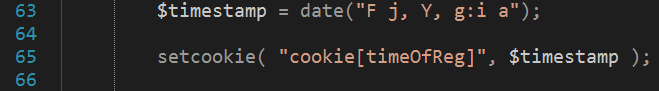
\includegraphics[width=1\textwidth]{img/vincent/abb18.png}
\newline
Wie aus dem Coding zu entnehmen ist, wurde dabei der Zeitpunkt der Registrierung im Cookie gespeichert. Das Auswerten des Cookies findet beim erneuten Aufruf der Website statt:
\newline
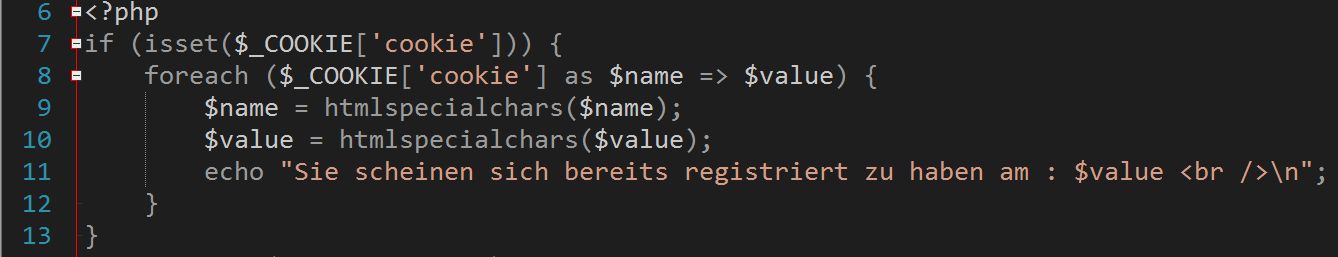
\includegraphics[width=1\textwidth]{img/vincent/abb19.png}
\newline
Dem User wird angezeigt, ob er sich mit hoher Wahrscheinlichkeit schon registriert hat, zus\"atzlich wird der Zeitpunkt der Registrierung ausgegeben. Folgendes Ergebnis wird dem User angezeigt:
\newline
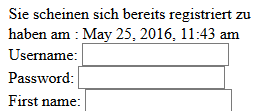
\includegraphics[width=0.6\textwidth]{img/vincent/abb20.png}
\newline

\chapter{Fazit}
\label{Fazit}
Trotz der Vielfalt der Anforderungen an die Website ist es durch dieses umfangreichere Projekt mehr oder weniger garantiert, ein Grundverständnis für die verwendeten Technologien zu entwickeln. 
\par
Durch die hohe Anzahl an unterschiedlichen, technologischen Anforderungen wird allerdings auch sehr schnell deutlich: Es gibt Technologien, welche sich relativ unkompliziert umsetzen lassen, und welche, die umfangreicher und wesentlich zeitaufwändiger sind. 
\par
Folglich reicht für ersteres ein Grundverständnis vollkommen aus. Ein Beispiel hierzu bietet das Heise Plug-In: Durch ein kleines Skript und einem zugehörigen HTML-Element ist das Plug-In schon komplett eingebunden. Die Funktionen des Plug-Ins können mit dem Grundverständnis darüber vollkommen ausgeschöpft werden.
\par
Anders hingegen ist das bei komplexeren Anforderungen, wie z.B. node.js oder Google Maps. Mit einem Grundverständnis lassen sich zwar einigermaßen schnell eine Datenbankverbindung, ein Server oder eine Karte erstellen - jedoch sind node.js und die Google Maps API wesentlich mächtiger und umfangreicher. 
\\
Mit node.js können bspw. \textit{"'Connection-Pools"'} zur Optimierung von gleichzeitigen Datenbankverbindungen verwendet werden und Websockets aufgebaut werden. 
\\
Die API von Google Maps bietet umfassendere Kartenfunktionen, wie Streetview oder Satellitenkarten.
\\
Bei solchen Anforderungen ist ein fundiertes Wissen über diese Technologien von Nöten, um sie wirklich meistern zu können.
